%%%%%%%% SD4H @ ICML 2026 — Workshop Draft v7 %%%%%%%%%%%%%%%%%%
% v7: Compressed to 4-page main-text limit (excl. refs/appendix).
%     Science unchanged from v6; trimmed Methods data-acquisition,
%     Results per-subject blurbs, Discussion Limitations/Related.

\documentclass{article}

\usepackage{microtype}
\usepackage{graphicx}
\usepackage{subcaption}
\usepackage{booktabs}
\usepackage{hyperref}

\newcommand{\theHalgorithm}{\arabic{algorithm}}

\usepackage{icml2026}

\usepackage{amsmath}
\usepackage{amssymb}
\usepackage{mathtools}
\usepackage{xcolor}
\usepackage{multirow}

\usepackage[capitalize,noabbrev]{cleveref}

% Placeholder command for figures not yet created
\newcommand{\figplaceholder}[2]{%
  \begin{center}
    \fbox{\parbox{#1}{\centering\vspace{1.5em}\textcolor{gray}{\textbf{[FIGURE PLACEHOLDER]}\\#2}\vspace{1.5em}}}
  \end{center}
}

\icmltitlerunning{Inferring Low-Dimensional Distortion Fields from Structured Neural Representations}

\begin{document}

\twocolumn[
  \icmltitle{Inferring Low-Dimensional Distortion Fields from \\
    Structured Neural Representations}

  \icmlsetsymbol{equal}{*}

  \begin{icmlauthorlist}
    \icmlauthor{Anonymous Authors}{anon}
  \end{icmlauthorlist}

  \icmlaffiliation{anon}{Anonymous Institution}

  \icmlcorrespondingauthor{Anonymous Author}{anonymous@example.com}

  \icmlkeywords{structured representation, individualized phenotype inference, representational geometry, color vision deficiency, fMRI}

  \vskip 0.3in
]

\printAffiliationsAndNotice{}

%==============================================================================
\begin{abstract}
%==============================================================================
Many health conditions manifest as structured distortions in high-dimensional biological representations, yet inferring these distortions in an interpretable and individualized manner remains challenging.
Here we present a framework for inferring low-dimensional distortion fields from structured neural representations, using color vision deficiency (CVD) as a case study.
From fMRI-measured hue representations in visual cortex, we extract a geometry-sensitive phenotype---the interpolation vulnerability profile---and invert it into parsimonious, mechanistically interpretable distortion parameters (1--2 DOF).
Applied to three Ishihara-confirmed CVD participants, the framework recovers subject-specific distortion fields: a 1-parameter retinal cone-shift for moderate protanomaly and a 2-parameter retinal--cortical model for mild deuteranomaly.
A third deutan case returns a null fit at both the LOCO and SRM representational levels and is reserved as a future-work probe of alternative representational dimensions.
Retinal and cortical models converge on detection but prescribe divergent corrections, generating falsifiable behavioral predictions.
\end{abstract}

%==============================================================================
\section{Introduction}
\label{sec:intro}
%==============================================================================

Many health conditions manifest as structured distortions in high-dimensional biological data---not as random noise or complete signal loss, but as systematic geometric deformations of the underlying representation.
Inferring these distortions in an interpretable and individualized manner is a key challenge for personalized intervention: the distortion must be mapped to a low-dimensional, mechanistically meaningful parameter space that can inform intervention design.

Color vision deficiency (CVD) provides a tractable case study for this problem.
CVD arises from altered spectral sensitivity of retinal cone photoreceptors, affecting approximately 8\% of males \citep{machado2009}, and produces structured distortions in cortical color representations that vary across individuals.
Current assistive approaches, including commercial spectral-notch filters, apply a fixed, generic correction; recent evidence indicates that such filters alter color \emph{appearance} but have minimal effect on color \emph{discrimination} at threshold \citep{somers2024}, suggesting that effective correction may require individually-tailored strategies.

The functional deficit that matters for continuous color tasks is not categorical classification but whether the continuous geometry between hues is preserved, and cortical compensation varies substantially even within a diagnostic category \citep{tregillus2021}.
We therefore treat fMRI responses as \emph{structured neural representations} whose relational geometry can be inverted into low-dimensional latent distortion parameters.

Here we present a framework that extracts a geometry-sensitive phenotype from structured neural representations and inverts it into parsimonious, interpretable distortion fields.
The unit of inference is the individual distortion field, not the population mean.
Our contributions are:
\begin{enumerate}
    \item We formulate distorted neural geometry as a structured representation inference problem and derive a geometry-sensitive phenotype---the interpolation vulnerability profile---that captures subject-specific structural deficits beyond classification accuracy.
    \item We infer low-dimensional, interpretable distortion parameters (1--2 DOF) from high-dimensional neural representations, showing that different CVD individuals require different parsimonious models within a closed-testing escalation.
    \item We show that the inferred distortion fields generate level-specific, falsifiable correction predictions: retinal and cortical models prescribe divergent corrections whose behavioral adjudication constitutes a concrete future test design.
\end{enumerate}

%==============================================================================
\section{Methods}
\label{sec:methods}
%==============================================================================

\subsection{Data Acquisition and Structured Representation}

Ten participants (7 HC; 3 CVD, all Ishihara-confirmed: two deutan, one protan) viewed eight colors equally spaced in CIE~$L^*a^*b^*$ ($L^* = 75$, chroma 40) across six 3T-fMRI runs using a modified RSVP paradigm \citep{brouwer2009}.
Functional images were preprocessed with fMRIPrep, projected to retinotopic ROIs (V1, V2, hV4) via the Wang atlas \citep{wang2015}, and summarized as Procrustes-aligned per-color amplitudes (see App.~\ref{app:supporting}).
Given the small CVD sample, all CVD results are interpreted as individual case demonstrations \citep{crawford1998}.

We modeled hue-selective neural populations with half-wave rectified squared sinusoidal basis functions \citep{brouwer2009} ($K$ channels), with the channel-to-voxel weight matrix $W$ estimated via ridge regression with GCV regularization \citep{golub1979}.
This encoding model transforms raw voxel data into a structured representation in which the relational geometry across hues is explicitly parameterized.

\subsection{Structured Phenotype Extraction: Interpolation Vulnerability}

The target phenotype is the \emph{LOCO vulnerability profile}, a geometry-sensitive summary of the structured representation.
Leave-one-color-out (LOCO) cross-validation tests whether the encoding model can interpolate to novel hues: $W$ is trained on 7 of 8 colors and prediction error for the held-out color is recorded.
The per-color errors define an 8-element vulnerability vector $\mathbf{v} \in \mathbb{R}^8$ for each participant, capturing which hues are poorly interpolated from their neighbors---a structural deficit invisible to classification-based decoders.

This phenotype is specific to continuous geometry: leave-one-\emph{run}-out (LORO) classification shows no HC--CVD difference ($p = 0.668$), while LOCO interpolation error is significantly elevated in CVD.
Among the ROIs tested, the effect was most robust in hV4 ($p = 0.017$; $K{=}3$), consistent with hV4's established role in perceptual color representation \citep{brouwer2009, bannert2018}.
We therefore focus distortion inference on hV4, with V1 analyses reported as cross-ROI validation in \cref{app:supporting}.

A complementary 28-dimensional summary is the pairwise representational distance matrix (RDM) of crossnobis distances, with $\Delta\text{RDM} = \text{RDM}_{\text{CVD}} - \overline{\text{RDM}}_{\text{HC}}$ capturing deviation from the HC mean; it enters fitting as a regularizer (\cref{eq:loss}) and provides an independent cross-criterion test in V1.

\subsection{Inverse Inference of Low-Dimensional Distortion Fields}

Given the structured phenotype $\mathbf{v}$, we infer the low-dimensional distortion parameters that best explain it.
We test two mechanistically distinct model families (\cref{fig:main}a), each parameterizing how a physical stimulus angle $\theta$ is transformed into a distorted angle $\theta'$.
The first family targets retinal-level distortion; the second targets cortical opponent-axis reorganization.
Within the cone-based family, the 1-DOF model and the 2-DOF extension are tested.
Because the two families address different scientific questions---retinal origin vs.\ cortical compensation---they are reported separately, with cross-family convergence interpreted as dual-level evidence.

\paragraph{Family 1: Cone-based models (retinal origin).}

\paragraph{Machado cone shift (1 DOF).}
A physiological model \citep{machado2009} in which the anomalous cone's spectral peak is shifted by $\Delta\lambda \in [0, 20]$~nm, predicting hue distortion through altered L--M cone opponency.

\paragraph{Retinal + cortical gain (R+C; 2 DOF).}
Extends the cone shift with a cortical opponent-channel gain $g$:
\begin{equation}
rg' = rg_{\text{base}} + (1{+}g) \cdot (rg_{\text{ret}} - rg_{\text{base}})
\label{eq:rc}
\end{equation}
where $g{=}0$ reduces to pure Machado, $g{=}{-}1$ is exact cortical compensation, and $g{<}{-}1$ is overcompensation \citep{tregillus2021}.

\paragraph{Family 2: Cortical opponent-axis model.}
As a complementary cortical-level analysis, we fit a 2-component angular dilation model (2 DOF) that parameterizes distortion along two opponent axes in hue space:
\begin{equation}
\theta'(c) = \theta(c) + \beta_s \cos(\theta(c) {-} 90^\circ) + \beta_c \cos(\theta(c) {-} \theta_{\text{conf}})
\label{eq:2comp}
\end{equation}
where $\beta_s$ captures S-cone axis expansion and $\beta_c$ captures confusion-axis modulation ($\theta_{\text{conf}} = 16^\circ$ for protan, $150^\circ$ for deutan).
This model is additionally validated against pairwise representational distance matrices ($\Delta$RDM) in V1.

\subsection{Specificity and Validation}

For each model and candidate parameter(s), we simulate the vulnerability profile that a healthy observer would exhibit if viewing stimuli distorted by the model's forward map.
Parameters are selected by minimizing a composite loss that respects two complementary geometric properties: per-color functional vulnerability and pairwise representational structure:
\begin{equation}
L_{\text{fit}} = \underbrace{\alpha \, L_{\text{vuln}} + \beta \, L_{\text{rank}}}_{\text{per-color (8-dim)}} + \underbrace{\delta \, L_{\text{rdm}}}_{\text{pairwise (28-dim)}} + \epsilon \, L_{\text{smooth}}
\label{eq:loss}
\end{equation}
where $L_{\text{vuln}}$ is MSE between simulated and observed profiles, $L_{\text{rank}} = 1 - \rho$ penalizes rank disagreement, $L_{\text{rdm}}$ encourages pairwise distance coherence, and $L_{\text{smooth}}$ regularizes adjacent-color shifts ($\alpha{=}1.0$, $\beta{=}0.5$, $\delta{=}0.2$, $\epsilon{=}0.1$; per-color terms dominate).
Effective DOF are 1--2, well below data dimensionality of 8; parameters are optimized over grids.
Statistical significance is assessed by exact permutation of the 8-color labels ($8! = 40{,}320$) on the Spearman $\rho$ between the best-fit simulated and observed vulnerability vectors.
A valid model must reach significance ($p < 0.05$) on the per-color vulnerability profile; HC-based false-positive calibration is reported separately in \cref{app:hc_specificity}.

%==============================================================================
\section{Results}
\label{sec:results}
%==============================================================================

\subsection{Subject-Specific Distortion Inference}

\cref{tab:main} and \cref{fig:main} present the central result: the framework infers distinct low-dimensional distortion fields for two of the three Ishihara-confirmed CVD participants, while the third (Sub-10, deutan) is null at both the LOCO and SRM representational levels used here.

\begin{table}[t]
  \caption{Inferred distortion parameters (hV4 LOCO, cone-based family). Within the cone-based family, the 1-DOF Machado model is tested first; the 2-DOF R+C is tested only if Machado is non-significant (closed testing). Sub-10 is null at this representational level (LOCO and SRM).}
  \label{tab:main}
  \begin{center}
    \begin{small}
      \begin{tabular}{llcccc}
        \toprule
        Subject & Model & DOF & $\rho$ & $p_{\text{perm}}$ \\
        \midrule
        Sub-08 (deutan) & R+C & 2 & 0.857 & \textbf{0.005**} \\
        Sub-09 (protan) & Machado & 1 & 0.762 & \textbf{0.018*} \\
        Sub-10 (deutan) & --- & --- & $-0.048$ & 0.559 \\
        \bottomrule
      \end{tabular}
    \end{small}
  \end{center}
  \vskip -0.15in
\end{table}

\textbf{Sub-09 (moderate protanomaly).}
The 1-DOF Machado model with $\Delta\lambda = 13.5$~nm---within the established range for moderate--severe protanomaly \citep{machado2009}---captures the profile at $\rho = 0.762$, $p = 0.018$; adding the cortical gain does not improve fit ($g = 0.0$ at optimum).

\textbf{Sub-08 (mild deuteranomaly).}
Machado is trend-level ($p = 0.058$); under the pre-specified closed testing, we escalate to R+C, which with $\Delta\lambda = 2.0$~nm and $g = +2.25$ reaches $\rho = 0.857$, $p = 0.005$.
The retinal shift alone explains little of this participant's distortion.

\textbf{Sub-10 (deutan).}
Cone-level models yield $\Delta\lambda \approx 0$ ($p = 0.559$) and the SRM criterion is also null; this outcome bounds the sensitivity of the LOCO/SRM representational levels rather than evidencing specificity against healthy vision, and is reserved as a future-work probe of alternative representational dimensions.

\begin{figure}[t]
  \centering
  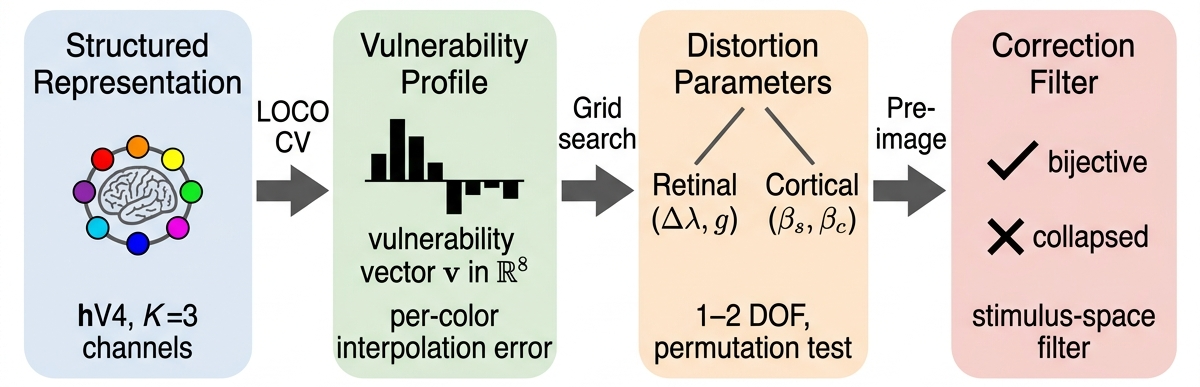
\includegraphics[width=0.92\columnwidth]{figures/fig1a_pipeline.png}\\[0.1em]
  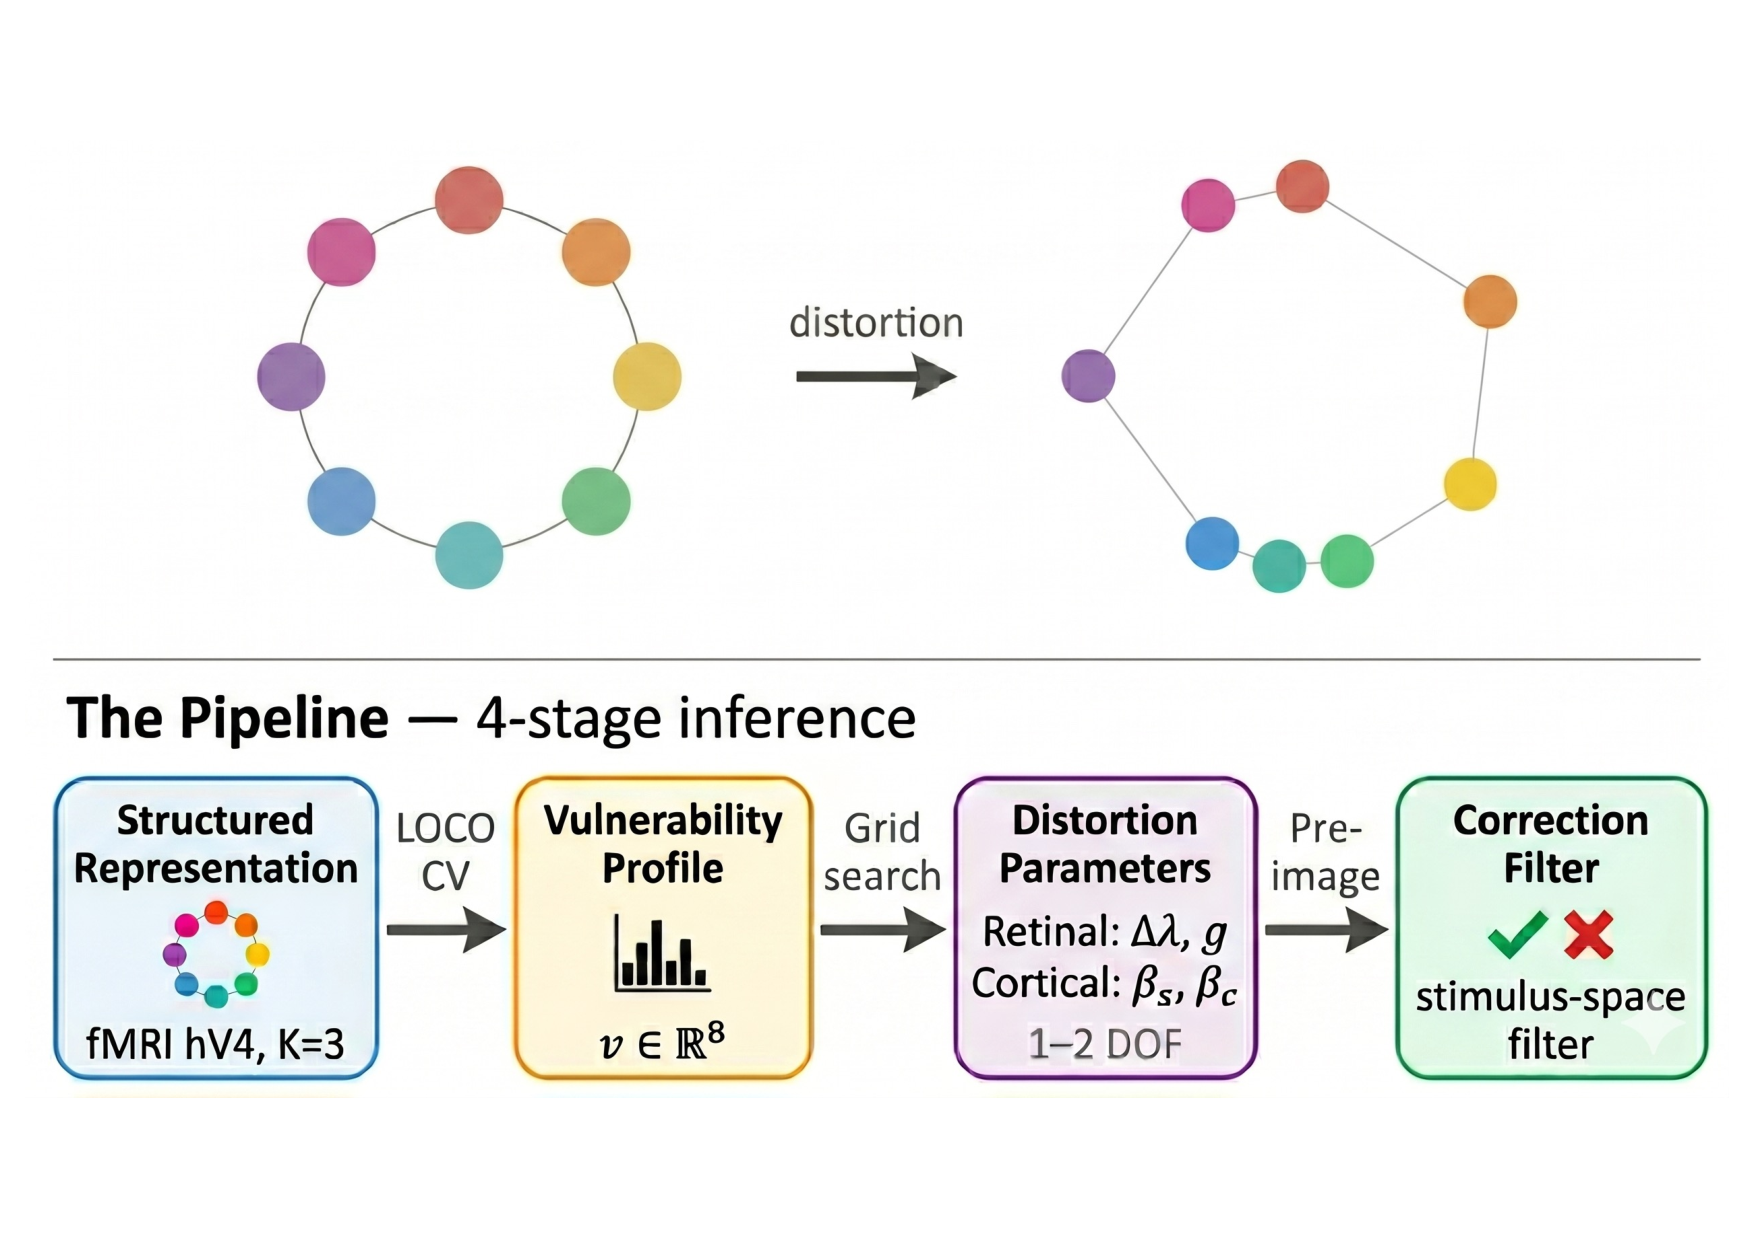
\includegraphics[width=\columnwidth]{figures/fig1_panels_bcd.pdf}
  \caption{The framework infers subject-specific distortion fields from structured neural representations. \textbf{(a)} Pipeline: structured representation $\to$ geometry-sensitive phenotype (LOCO vulnerability) $\to$ inverse inference of distortion parameters $\to$ correction assessment. \textbf{(b--d)} 8-color LOCO vulnerability profiles. Gray bars: observed CVD profile; colored line: best-model fit. \textbf{(b)} Sub-08: R+C ($\rho{=}0.857$, $p{=}0.005$). \textbf{(c)} Sub-09: Machado ($\rho{=}0.762$, $p{=}0.018$). \textbf{(d)} Sub-10: flat profile, $p{=}0.559$ (null at LOCO/SRM levels).}
  \label{fig:main}
  \vskip -0.15in
\end{figure}

\subsection{Interpretability of Inferred Parameters}

The inferred retinal parameters fall within established physiological ranges \citep{machado2009}: sub-09's $\Delta\lambda = 13.5$~nm (moderate protanomaly, $g{=}0$, purely retinal) and sub-08's $\Delta\lambda = 2.0$~nm (mild deuteranomaly).
Sub-08's cortical gain ($g = +2.25$) may reflect cortical amplification of a weak retinal signal, though it could also absorb unmodeled variance; we treat it as a provisional effective description (see \cref{app:supporting}).

\subsection{Convergent Detection, Divergent Correction}

The cortical-level 2-component model (\cref{eq:2comp}) also reaches significance in hV4 for both fit-recovered participants: sub-08 ($\beta_s = 38^\circ$, $\beta_c = -14^\circ$; $\rho = 0.881$, $p = 0.004$) and sub-09 ($\beta_s = 6^\circ$, $\beta_c = -22^\circ$; $\rho = 0.690$, $p = 0.035$); sub-10 is trend-level under this model ($p = 0.058$) but remains null at the primary LOCO criterion.
The two families \emph{converge on detection}---both identify the same two individuals as distorted---but \emph{diverge on correction}: for sub-08, the cone-based and cortical models prescribe correction directions with cosine $= -0.18$ (sign agreement 3/8), despite comparable fit quality ($\rho = 0.857$ vs.\ $0.881$).
This divergence is a falsifiable prediction: the retinal model prescribes spectral pre-distortion, while the cortical model prescribes opponent-axis rescaling; a behavioral 2AFC task would simultaneously validate the correction and localize the dominant processing level.

Correction feasibility is severity- and level-dependent: the retinal model admits exact pre-image inversion for sub-08 but is irreversible for sub-09 (4/8 colors merge under arc compression), while the cortical model preserves bijectivity for both (details in \cref{app:supporting}).

When fitted independently to V1 $\Delta$RDM, the S-cone parameter converges at ${\sim}21.5^\circ$ across both CVD participants, matching the $21.4^\circ$ from behavioral hue-scaling \citep{emery2021}---suggesting a shared compensatory mechanism \citep{tregillus2021, boehm2014}.

%==============================================================================
\section{Discussion}
\label{sec:discussion}
%==============================================================================

\paragraph{Geometry-sensitive sufficient statistics.}
Classification accuracy is sufficient for categorical identity but discards the continuous relational geometry needed to detect structured distortion.
The LOCO profile compresses voxel data into an 8-element geometric summary, and the composite loss (\cref{eq:loss}) decomposes fidelity into per-color (8-dim) and pairwise (28-dim) components---an approach that may generalize to other conditions where sensory representations are distorted rather than absent.

\paragraph{What this framework does not establish.}
We have \emph{not} shown that the resulting corrections improve perceptual discrimination---that requires behavioral validation, and the divergent correction predictions from the two model families constitute the framework's primary testable output.

\paragraph{Limitations.}
Three CVD participants and fMRI dependence make this a proof-of-concept, not a screening tool; with DOF $\leq 2$ on 8 data points, rank-based grid optimization yields an elevated HC false-positive rate (15/21, see \cref{app:hc_specificity}).
The two fit-recovered CVD cases are distinguished from HC fits by physiologically interpretable parameters and cross-criterion convergence (\cref{tab:full}); Sub-10 is null at both LOCO and SRM.
Since this is an individual-profiling pipeline for \emph{known} CVD cases, we do not claim specificity against healthy vision from this case series.

%==============================================================================
\section{Conclusion}
\label{sec:conclusion}
%==============================================================================

We present a framework for inferring low-dimensional distortion fields from structured neural representations, demonstrated on CVD.
By extracting a geometry-sensitive phenotype invisible to classification accuracy and inverting it into parsimonious mechanistic parameters, the framework recovers subject-specific distortion fields at two processing levels that converge on detection but diverge on correction---generating falsifiable behavioral predictions as the immediate next step.

%==============================================================================
\section*{Impact Statement}
%==============================================================================

This work develops personalized inference methods for characterizing sensory distortion from structured neural data, with color vision deficiency as the initial application.
Potential positive impacts include individually-tailored color corrections for digital displays and accessibility tools.
The framework currently requires fMRI data, limiting immediate clinical deployment.
Behavioral validation and informed consent are essential prerequisites before any correction is applied, as a misspecified model could impair rather than improve visual function.

%==============================================================================
\bibliography{genbio_draft_v5}
\bibliographystyle{icml2026}

%==============================================================================
%==============================================================================
\newpage
\appendix
\onecolumn

\section{Supporting Analyses}
\label{app:supporting}

\subsection{HC Specificity Calibration}
\label{app:hc_specificity}

To empirically calibrate the false-positive rate of the grid-search fitting procedure, we applied the full hV4 LOCO pipeline to all 7 HC participants, treating each as if they were a CVD candidate (best-family selected per model).

\paragraph{Results.}
\cref{tab:hc_fpr} reports the number of HC participants reaching $p < 0.05$ for each model.
The observed false-positive rate substantially exceeds the nominal 5\%: 15/21 model--subject tests are significant, compared to the expected 1.05 under the null.
The 2-component model is worst (7/7), Machado is least inflated (3/7).

\begin{table}[h]
  \caption{HC false-positive rates (hV4 LOCO, $p < 0.05$).}
  \label{tab:hc_fpr}
  \begin{center}
    \begin{small}
      \begin{tabular}{lccc}
        \toprule
        Model & DOF & HC significant & FPR \\
        \midrule
        Machado & 1 & 3/7 & 43\% \\
        R+C & 2 & 5/7 & 71\% \\
        2-Component & 2 & 7/7 & 100\% \\
        \midrule
        Total & & 15/21 & 71\% \\
        \bottomrule
      \end{tabular}
    \end{small}
  \end{center}
\end{table}

\begin{figure}[h]
  \centering
  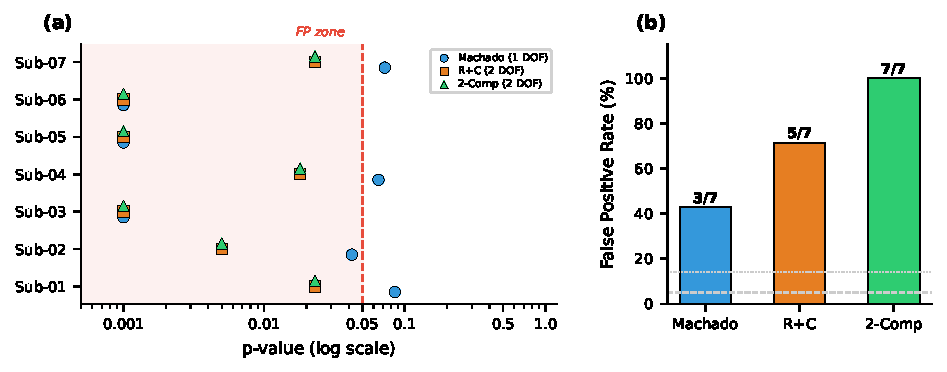
\includegraphics[width=\textwidth]{figures/fig_hc_specificity.pdf}
  \caption{HC specificity calibration. \textbf{(a)} Per-subject p-values for each model (log scale). The red dashed line marks $\alpha = 0.05$; shaded region indicates the false-positive zone. \textbf{(b)} Aggregate false-positive rates. Dashed line: nominal $\alpha = 5\%$; dotted line: chance rate for $n{=}7$ (14.3\%). Higher model complexity (DOF) yields higher false-positive rates.}
  \label{fig:hc_specificity}
\end{figure}

\paragraph{Mechanism.}
The elevated FPR arises from two reinforcing factors:
\begin{enumerate}
\item \textbf{Grid-search flexibility on 8 data points.} With 1--2 DOF optimized over a fine grid (41--1,326 candidate parameter configurations) and rank-based loss ($L_{\text{rank}} = 1 - \rho$), most individuals---healthy or not---will have some configuration that achieves a nominally significant rank correlation with 8 elements. This is a known property of permutation tests under flexible model search.
\item \textbf{Regression to the mean.} HC individuals with low baseline LOCO performance (i.e., already poorly interpolated before any model fitting) have the most room for apparent improvement. We observe a strong negative correlation ($r = -0.894$) between HC baseline $\rho$ and the improvement $\Delta\rho$ achieved by fitting, confirming that the signal captured in HC fits is predominantly regression to the mean rather than color-specific structure.
\end{enumerate}

\paragraph{Why this does not invalidate the fit-recovered CVD results.}
The pipeline is designed for \emph{individual profiling} of known CVD cases, not population screening; we do not claim specificity against healthy color vision from the present case series.
The two fit-recovered CVD cases are distinguished from HC fits by three properties absent in HC:
(i) inferred parameters fall within established physiological ranges (Sub-09 $\Delta\lambda = 13.5$~nm matches moderate protanomaly; Sub-08 $\Delta\lambda = 2.0$~nm matches mild deuteranomaly);
(ii) the 2-component model shows cross-criterion convergence (LOCO and $\Delta$RDM both significant for both fit-recovered participants; no HC achieves this); and
(iii) $\beta_s \approx 21.5^\circ$ converges with an independent behavioral estimate \citep{emery2021}.
In sum, HC fits reflect opportunistic overfitting to 8 data points, whereas the fit-recovered CVD cases align with convergent external evidence.
Sub-10 is Ishihara-confirmed CVD but is null at both the LOCO and SRM representational levels used here; probing this case at alternative representational dimensions is an explicit future-work direction.

\subsection{Cross-ROI and Cross-Criterion Evidence}

Beyond the primary hV4 LOCO inference, the 2-component model was validated across multiple ROIs and criteria.
Sub-08 V1 LOCO reached $p = 0.001$ ($\beta_s = 50^\circ$, $\beta_c = -14^\circ$)---the strongest LOCO result in the pipeline.
Sub-09 V1 $\Delta$RDM reached $p = 0.007$ (crossnobis cosine).
The 2-component model is the only model achieving significance under both LOCO and $\Delta$RDM criteria for both CVD participants (\cref{tab:full}).

\subsection{Model-Dependent Correction Feasibility}

\begin{figure}[h]
  \centering
  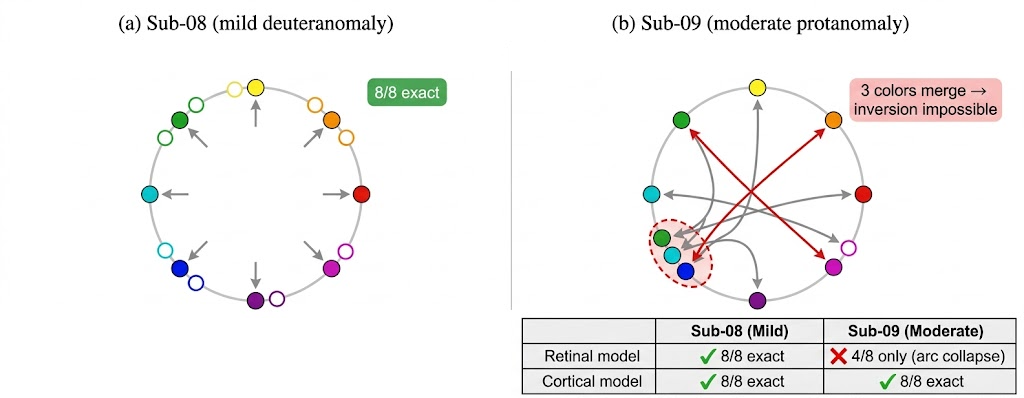
\includegraphics[width=\textwidth]{figures/fig2_collapse.png}
  \caption{Correction geometry depends jointly on severity and modeling level. \textbf{(a)} Mild distortion (Sub-08): wide opponent arc preserved; all 8 colors admit exact pre-image inversion ($<0.001^\circ$ error). \textbf{(b)} Moderate distortion (Sub-09): arc compresses 360$^\circ \to \sim$96$^\circ$; three colors merge, making exact inversion impossible. The retinal model achieves exact correction only for mild distortion (4/8 for moderate), while the cortical 2-component model preserves bijectivity for both (bottom table).}
  \label{fig:feasibility}
\end{figure}

Under the cortical-level 2-component model, both CVD participants admit exact pre-image solutions for all 8 colors (sub-08: mean $|\delta| = 46.3^\circ$; sub-09: mean $|\delta| = 20.1^\circ$; residual $< 0.001^\circ$).
This contrasts with the retinal Machado model, where sub-09's arc compression makes exact inversion impossible for 4/8 colors.
The difference arises because angular dilation in opponent hue space preserves bijectivity by construction, whereas retinal spectral shifts can compress the opponent arc irreversibly.

For sub-08, the R+C and 2-component models prescribe substantially different correction directions (cosine between correction vectors = $-0.18$; sign agreement 3/8), despite comparable fit quality (R+C $\rho = 0.857$ vs.\ 2-component $\rho = 0.881$).
Which correction actually improves perception requires behavioral validation.

\subsection{Model Comparison: Full Table}

\begin{table}[h]
  \caption{Full model comparison across hV4 LOCO, V1 LOCO, and V1 $\Delta$RDM criteria. The 2-component model is the only model achieving significance under both LOCO and $\Delta$RDM for both CVD participants.}
  \label{tab:full}
  \begin{center}
    \begin{small}
      \begin{tabular}{llcccccc}
        \toprule
        Subject & Model & DOF & hV4 LOCO $\rho$ & hV4 LOCO $p$ & V1 LOCO $p$ & V1 $\Delta$RDM & Notes \\
        \midrule
        \multirow{3}{*}{Sub-08} & Machado & 1 & 0.619 & 0.058 & 0.033* & anti-corr. & Trending (hV4) \\
        & R+C & 2 & \textbf{0.857} & \textbf{0.005**} & 0.047* & 0.179 & hV4 primary \\
        & 2-Comp & 2 & 0.881 & 0.004** & \textbf{0.001***} & CI excl.\ 0 & Cross-criterion \\
        \midrule
        \multirow{3}{*}{Sub-09} & Machado & 1 & \textbf{0.762} & \textbf{0.018*} & 0.112 & $+0.091$ & hV4 primary \\
        & R+C & 2 & 0.762 & 0.018 & --- & 0.026* & $g{=}0$ (= Machado) \\
        & 2-Comp & 2 & 0.690 & 0.035* & 0.018* & \textbf{0.007***} & Cross-criterion \\
        \midrule
        Sub-10 & Cone-level & --- & $-0.048$ & 0.559 & --- & --- & Null at LOCO/SRM \\
        & 2-Comp & 2 & --- & 0.058$^\dagger$ & --- & --- & Trend-level \\
        \bottomrule
        \multicolumn{8}{l}{\small $^\dagger$ Trend-level 2-component fit while primary LOCO criterion is null; see Limitations discussion.} \\
      \end{tabular}
    \end{small}
  \end{center}
\end{table}

\subsection{Correction Feasibility Details}

\paragraph{Sub-08 (R+C pre-image).}
All 8 colors admit exact pre-image solutions (mean $|\delta| = 23.5^\circ$, max $= 42.9^\circ$, residual $< 0.001^\circ$).
The resulting 8-point lookup table is directly implementable on any digital display.

\paragraph{Sub-09 (Machado pre-image).}
At $\Delta\lambda = 13.5$~nm, the opponent-space arc compresses from 360$^\circ$ to $\sim$96$^\circ$.
Colors c4 (green), c5 (cyan), and c6 (blue) converge to a single perceived angle ($\sim$282$^\circ$).
Exact pre-image: 4/8 colors.
Separation-optimized fallback: min separation $1.03^\circ \to 5.76^\circ$ ($5.6\times$), mean separation $39.3^\circ \to 24.3^\circ$ (healthy: 70.7$^\circ$).

\paragraph{Sub-09 (2-component pre-image).}
All 8 colors admit exact pre-image solutions (mean $|\delta| = 20.1^\circ$, max $= 48.1^\circ$, residual $< 0.001^\circ$).
The cortical-level angular dilation preserves bijectivity, unlike retinal spectral shift, enabling exact correction where the Machado model predicts irreversible collapse.

\end{document}
